\documentclass[a4paper,12pt]{article}
\usepackage[utf8]{inputenc}
\usepackage{amsmath,amssymb,amsthm}
\usepackage{natbib}
\usepackage[margin=3cm]{geometry}
\usepackage{todonotes}
\usepackage{mathtools}
\usepackage{subfiles}
\usepackage{subcaption}
\usepackage{booktabs}
\usepackage{setspace}
\doublespacing
\def\sb#1{\textcolor{blue}{#1}}
\begin{document}
\title{Big Brother Is Watching : Using Digital Surveillance Tools for Near Real-Time Mapping of the Risk of International Infectious Disease Spread}
\author{ Sangeeta Bhatia, Anne Cori and Pierre Nouvellet}
\maketitle

\begin{abstract}
  In our increasingly interconnected world, it is crucial to
  understand the risk of an outbreak originating in one country/region
  and  spreading to the rest of the world. Rapid recognition and
  response to potential pandemics and emerging diseases have become
  essential global health priorities. Digital disease surveillance
  tools such as ProMed and HealthMap have the potential to serve as
  important early warning systems as well as complement the field
  surveillance data during an ongoing outbreak. While there are a
  number of systems that carry out digital disease surveillance, there
  is as yet a lack of tools that can compile and analyse the generated
  data to produce easily understood actionable reports. We present a flexible statistical model that uses different streams
  of data (such as disease surveillance data, mobility data etc.) for
  short-term incidence trend forecasting.
  The work presented here makes 2 key contributions:
  \begin{enumerate}
  \item In validating the model using data collected by ProMED and
    HealthMap during the 2014-2016 West African Ebola outbreak,
    we provide a realistic appraisal of the strengths and limitations
    of such data in incidence forecasting.
    \item We infer incidence trends at finer spatial scales from
      aggregated data. Our work shows how the data from
      event based surveillance systems (EBS) can complement the data
      collected from traditional
      public health infrastructure. During an
      ongoing crisis, combining data from different sources gives
      stakeholders a more complete picture.
  \end{enumerate}
\end{abstract}
\section{Introduction}
\section{Results}
\subsection{Incidence trends from different data sources}
We aggregated the WHO data to national level to compare the incidence
trends derived from the three different data sources (WHO, HealthMap
and ProMED). As can be seen in Figure~\ref{fig:incid_comp}, the incidence time series
of the three data sources were well
correlated. Figure~\ref{fig:corrplot} shows the strength of the
correlation between the data from the three different sources.

\begin{figure}
    \centering
        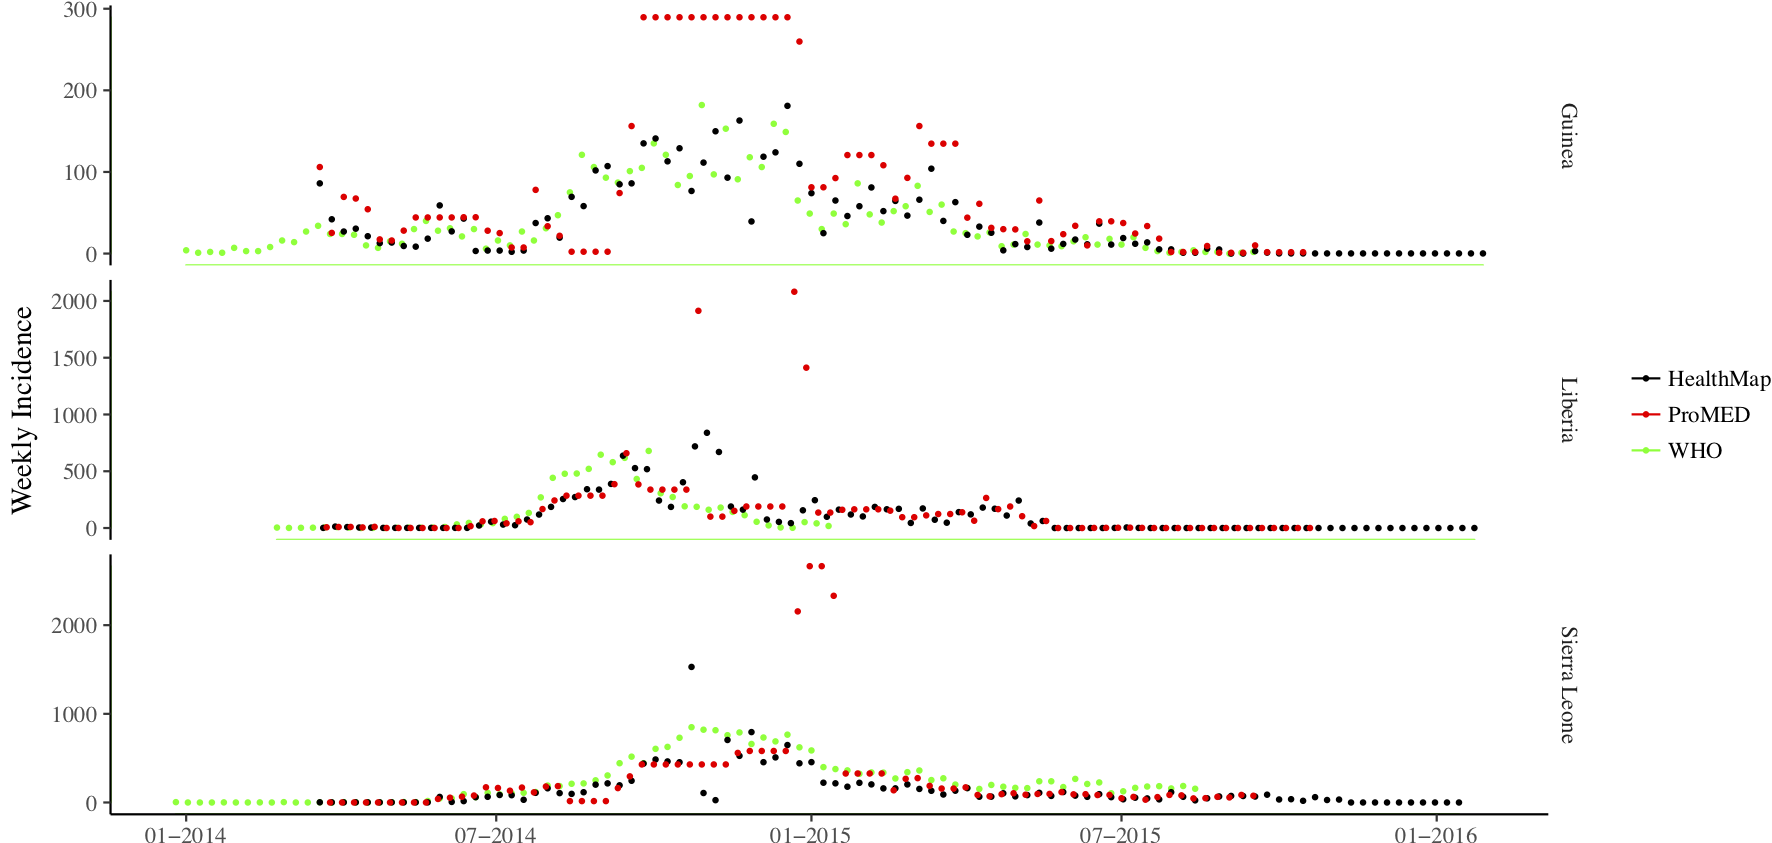
\includegraphics[width=\textwidth]{figures/who_hm_pm_weekly_incid-2}
        \caption{Comparison of weekly incidence data from WHO, HealthMap and ProMED.}
        \label{fig:incid_comp}
  \end{figure}


  \begin{figure}
    \centering
    \includegraphics[width=0.5\textwidth]{figures/correlation-matrix-2}
    \caption{Correlation matrix between the weekly incidence data from WHO,
      ProMED and HealthMap aggregated at country level. \textbf{The strength of the correlation is
      indicated by the size and colour of the circles.
      Deeper shades of blue indicate high correlation. The figure
      shows that the data collected by event based surveillance
      systems (ProMED and HealthMap) exhibit a
      high degree of correlation with the data collated by WHO
      indicating that  event based surveillance data are consistent with data
      from WHO.} All
      correlation coefficients were  highly statistically significant
      with p-value < 0.001.}
    \label{fig:corrplot}
  \end{figure}

  \sb{I think it would be good to compare monthly data from
   ProMED/HealthMap with corresponding data from WHO. The comparison
   above is for a post-hoc cleaned up data set from both.} 

 \subsection{Prediction using data from HealthMap and ProMED}
 Projections at different time steps using HealthMap and
 ProMED. (maybe 3).
 Show projections at different times in the same graph.

 \subsection{Prediction using data from WHO}
 Same as before. Note that there are 55 districts. It might not be
 useful to show 55 graphs (although others have done precisely this). 
 Also map from all districts showing uncertainty
 associated with predictions as discussed earlier.

 \subsection{Assessing Model Fit}
 \begin{enumerate}
 \item number of points within CI (predictive part).
 \item choose some test statistic that depends on the data or on data
   and parameters. For a large number of simulations, check where the
   observed statistic lie in the distribution of the simulated statistic (goodness-of-fit).
 \end{enumerate}
 
 \section{Using aggregate data to infer incidence in districts}

 Method 1. Take data from EBS and assign predictions to different
 districts in proportion to their relative population densities.
 Compare with data from WHO.

 \begin{figure}
   \centering
   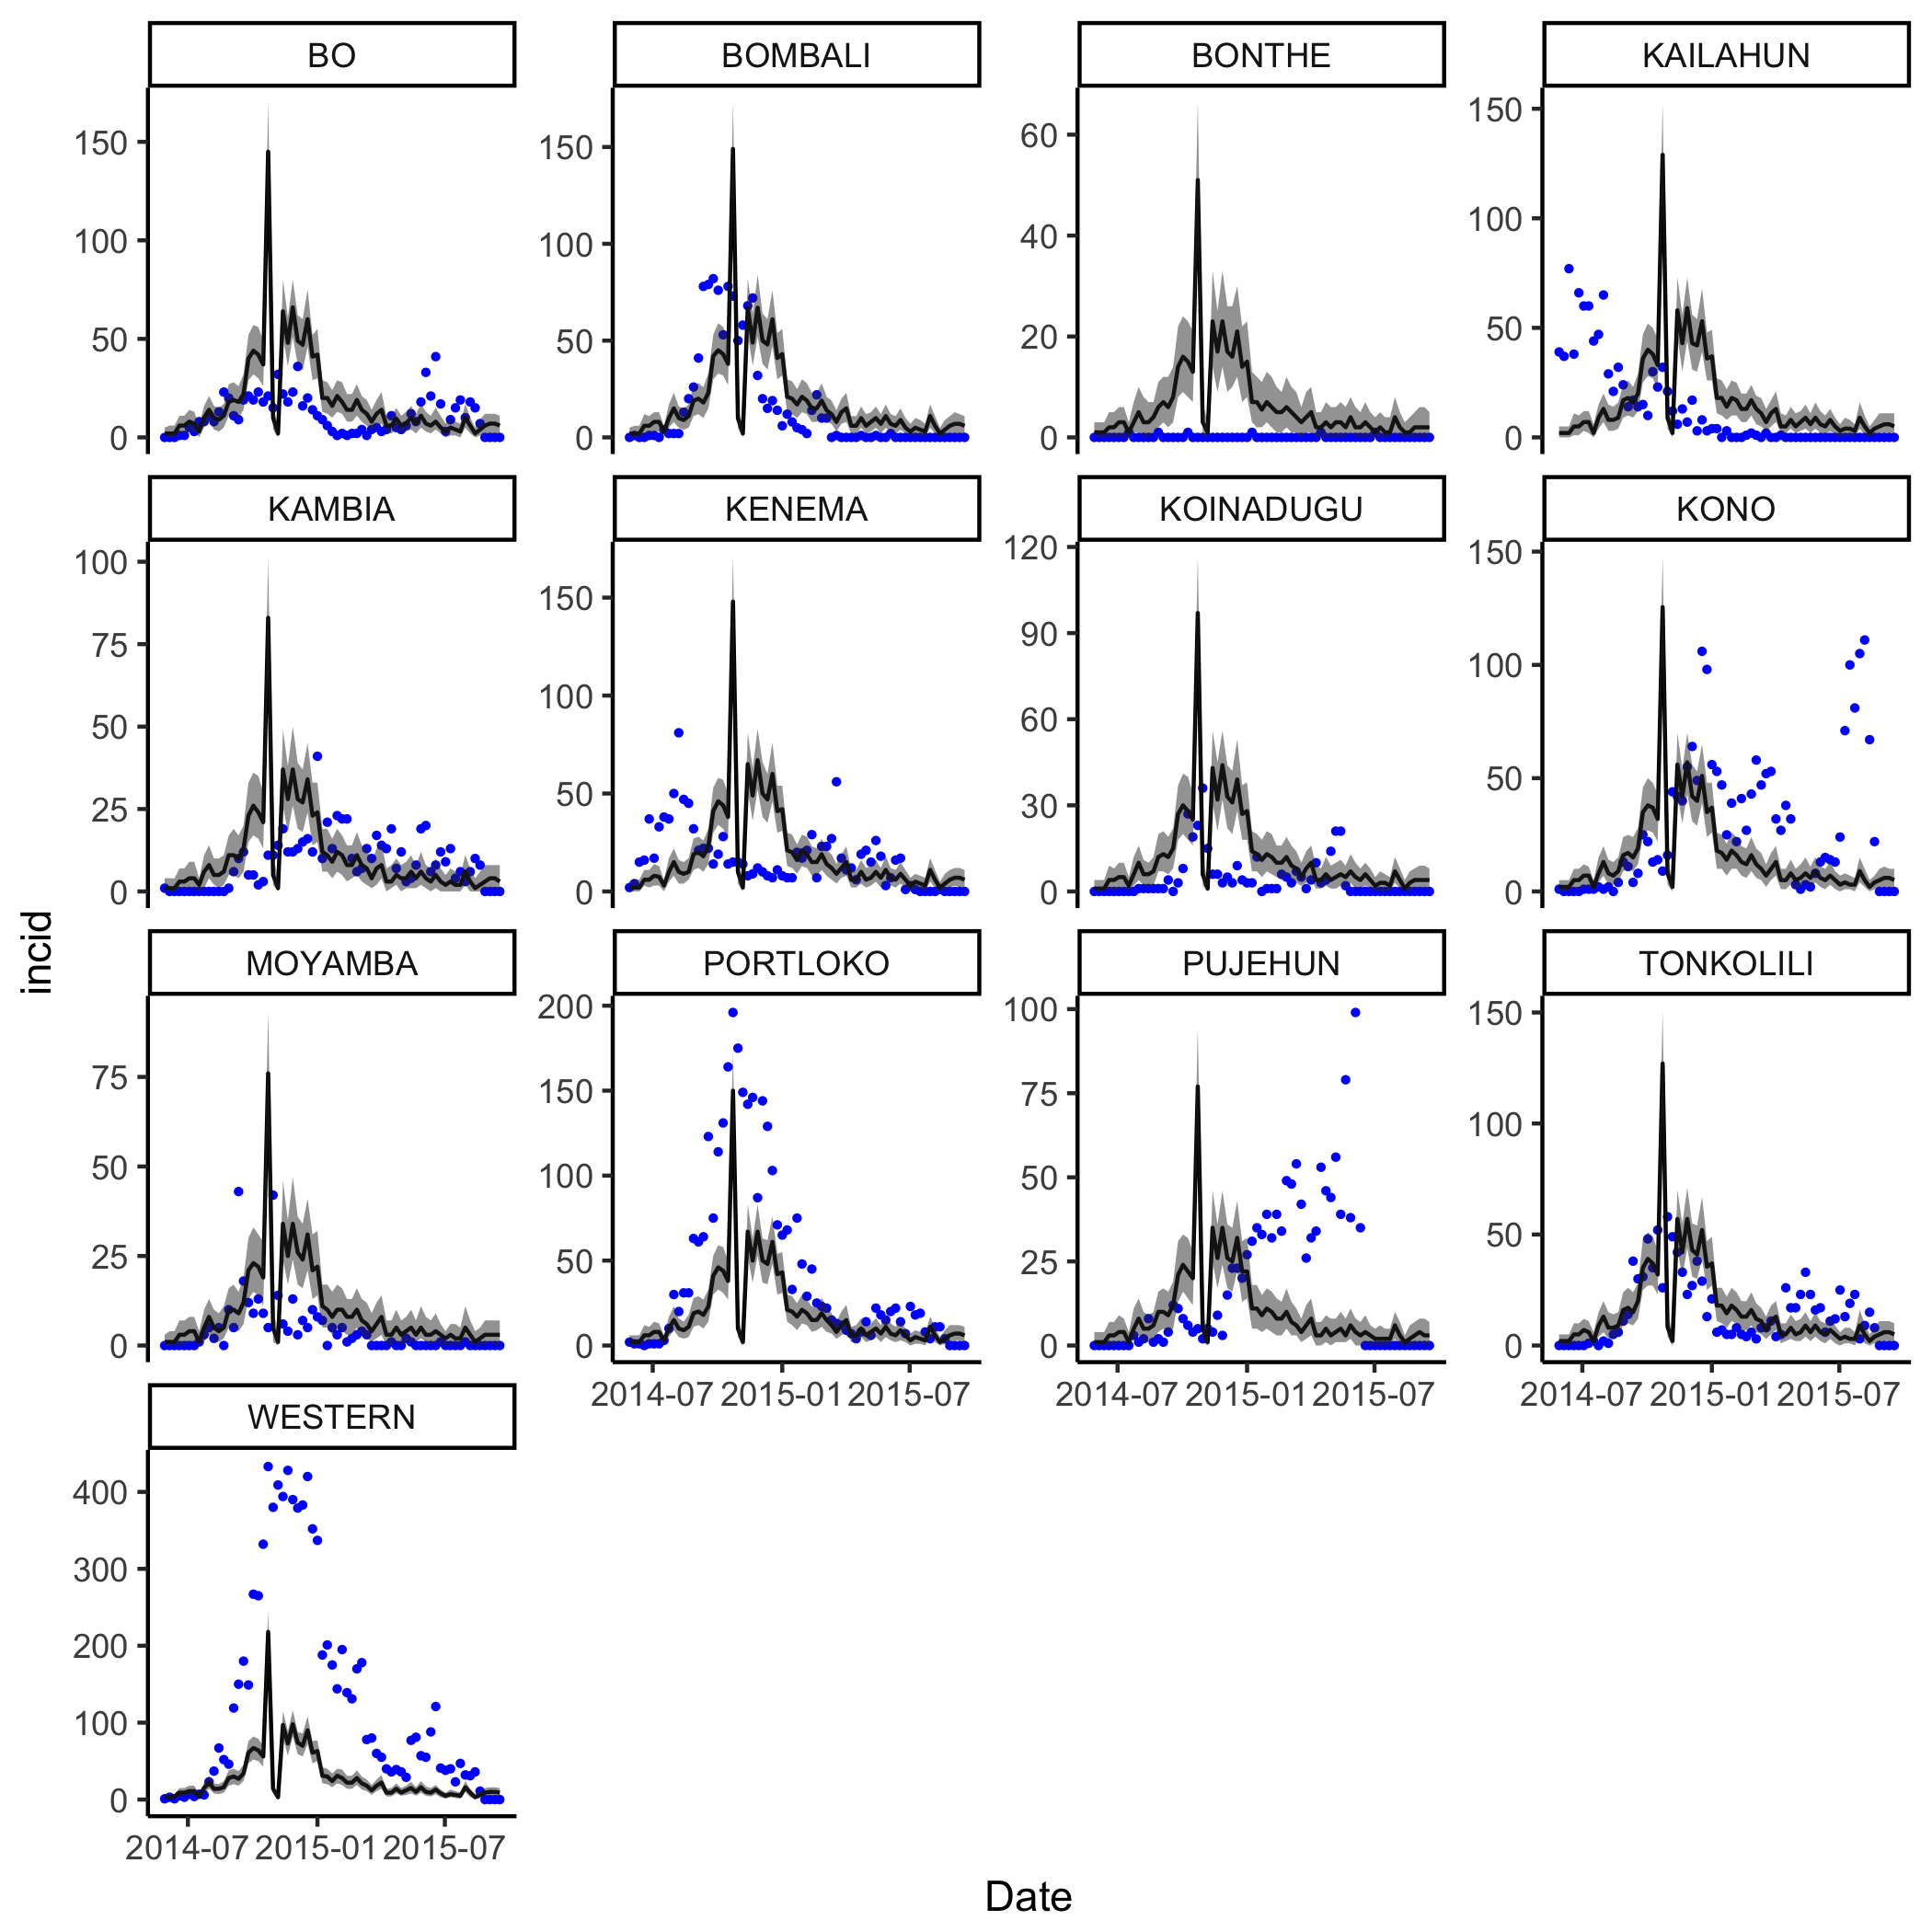
\includegraphics[width = \textwidth]{figures/disaggregation_1.png}
   \label{fig:disaggregate1}
   \caption{Assigning cases to districts in Sierra Leone with probabilities
     proportional to their relative population densities. In some
     districts such as Tonkolili and Bombali, the estimated case counts fit
     the observations (shown in blue) well whereas in other districts such as Western,
   the fit is very poor. This suggests while population density of a
   region is a key determinant of disease spread, other factors are at
 play that should be incorporated in the model. }
 \end{figure}

 \subsection{Discussion and future work}

 Opportunities - Integrating other data sources; choosing time
 window for reproduction number estimation.

 \section{Methods}
 \subsection{Model}
 The number of cases at a location \(j\) at time \(t\) is given by the equation
\[
  I_{j, t} \sim Pois\left( \sum_{i = 1}^{n} {\left( p_{i \rightarrow j}
  R_{t, i} \sum_{s = 1}^{t}{I_{i, t - s} w_{s}}\right)} \right),
\]

where \(R_{t, i}\) is the reproduction number at location \(i\) at time
\(t\) and \(p_{i \rightarrow j}\) is the probability of moving from
location \(i\) to location \(j\). The quantity $R_{t, i}$ is the
reproduction number at time $t$ at location $i$. $R_{t, i}$ is
affected by a number of other factors e.g., the intrinsic
transmissibility of a pathogen, the health care capacity at location
$i$ etc. Its dependence on these factors is formalized as
\[ R_{t, i} := f(haq_i, R_0, t),\]
where $haq_i$ is an index/score quantifying the health care capacity at location 
$i$, $f$ denotes a function, $R_0$ is the basic reproduction number (data stream 2) and $t$ is time..

The probability of moving between locations is derived from the
relative flow of populations.
This latter quantity is estimated using a population flow
model such as a gravity model \citep{grosche2007175}. Under a gravity model, the flow of individuals from area \(i\) to area \(j\),
\(\phi_{i \rightarrow j}\), is proportional to the product of the
populations of the two areas, \(N_i\) and \(N_j\) and inversely
proportional to the distance between them \(d_{i, j}\), all quantities
are raised to some power.
\[
  \phi_{i \rightarrow j} :=  \frac{N_i^{\alpha}N_j^{\beta}}{d_{i, j}^{\gamma}}.
\]

In practice, \( \alpha \) and \( \beta \) are assumed to be $1$. The
exponent \( \gamma \) modulates the effects distance on the flow of
populations. A large value of \( \gamma \) indicates that the
distances travelled by populations tend to be short.

The relative risk of spread at a location \(j\) from a location \(i\)
is thus the population flow into location \(j\) from location \(i\).

\[
  r_{i \rightarrow j}^{spread} = \frac{\phi_{i \rightarrow
  j}}{\sum_{x}{\phi_{i \rightarrow
  j}}}.
\]

The probability of movement from location \(i\) to location \(j\) is given by
\[  p_{i \rightarrow j} = (1 - p_{stay}^i) r_{i \rightarrow j}^{spread},\]

where \(p_{stay}^i\) is the probability of staying at location
\(i\). As the above equation indicates, by varying $p_{stay}^i$, we
can capture the dynamics of population flow across spatial units. For
instance, if \(p_{stay}^i\) is large, then the flow out of location
\(i\) would be small. Thus, if this parameter is geographically
heterogeneous, we obtain imbalanced flow of population (i.e. a source-sink dynamics). 

\subsection{Inference of model parameters}

MCMC simulation using Stan.
Show convergence statistics and other diagnostic information.

\section{Supplementary Information}
\subsection{Data pre-processing}
Information about the pre-processing steps and outlier removal.
\subsection{Sensitivity Analysis}
Some things to consider.
\begin{itemize}
\item What impact does changing priors for $\gamma$ have?
\item serial interval parameters?
  Changing the point of truncation? The time window?
\item changing exponents on population in the gravity model produces
  different behavior.
 \item maybe have another model of population flow.  
\end{itemize}
\bibliographystyle{plainnat}
\bibliography{mriids}
\end{document}